% Options for packages loaded elsewhere
\PassOptionsToPackage{unicode}{hyperref}
\PassOptionsToPackage{hyphens}{url}
\PassOptionsToPackage{dvipsnames,svgnames,x11names}{xcolor}
%
\documentclass[
  letterpaper,
  DIV=11,
  numbers=noendperiod]{scrartcl}

\usepackage{amsmath,amssymb}
\usepackage{iftex}
\ifPDFTeX
  \usepackage[T1]{fontenc}
  \usepackage[utf8]{inputenc}
  \usepackage{textcomp} % provide euro and other symbols
\else % if luatex or xetex
  \usepackage{unicode-math}
  \defaultfontfeatures{Scale=MatchLowercase}
  \defaultfontfeatures[\rmfamily]{Ligatures=TeX,Scale=1}
\fi
\usepackage{lmodern}
\ifPDFTeX\else  
    % xetex/luatex font selection
\fi
% Use upquote if available, for straight quotes in verbatim environments
\IfFileExists{upquote.sty}{\usepackage{upquote}}{}
\IfFileExists{microtype.sty}{% use microtype if available
  \usepackage[]{microtype}
  \UseMicrotypeSet[protrusion]{basicmath} % disable protrusion for tt fonts
}{}
\makeatletter
\@ifundefined{KOMAClassName}{% if non-KOMA class
  \IfFileExists{parskip.sty}{%
    \usepackage{parskip}
  }{% else
    \setlength{\parindent}{0pt}
    \setlength{\parskip}{6pt plus 2pt minus 1pt}}
}{% if KOMA class
  \KOMAoptions{parskip=half}}
\makeatother
\usepackage{xcolor}
\setlength{\emergencystretch}{3em} % prevent overfull lines
\setcounter{secnumdepth}{-\maxdimen} % remove section numbering
% Make \paragraph and \subparagraph free-standing
\makeatletter
\ifx\paragraph\undefined\else
  \let\oldparagraph\paragraph
  \renewcommand{\paragraph}{
    \@ifstar
      \xxxParagraphStar
      \xxxParagraphNoStar
  }
  \newcommand{\xxxParagraphStar}[1]{\oldparagraph*{#1}\mbox{}}
  \newcommand{\xxxParagraphNoStar}[1]{\oldparagraph{#1}\mbox{}}
\fi
\ifx\subparagraph\undefined\else
  \let\oldsubparagraph\subparagraph
  \renewcommand{\subparagraph}{
    \@ifstar
      \xxxSubParagraphStar
      \xxxSubParagraphNoStar
  }
  \newcommand{\xxxSubParagraphStar}[1]{\oldsubparagraph*{#1}\mbox{}}
  \newcommand{\xxxSubParagraphNoStar}[1]{\oldsubparagraph{#1}\mbox{}}
\fi
\makeatother


\providecommand{\tightlist}{%
  \setlength{\itemsep}{0pt}\setlength{\parskip}{0pt}}\usepackage{longtable,booktabs,array}
\usepackage{calc} % for calculating minipage widths
% Correct order of tables after \paragraph or \subparagraph
\usepackage{etoolbox}
\makeatletter
\patchcmd\longtable{\par}{\if@noskipsec\mbox{}\fi\par}{}{}
\makeatother
% Allow footnotes in longtable head/foot
\IfFileExists{footnotehyper.sty}{\usepackage{footnotehyper}}{\usepackage{footnote}}
\makesavenoteenv{longtable}
\usepackage{graphicx}
\makeatletter
\newsavebox\pandoc@box
\newcommand*\pandocbounded[1]{% scales image to fit in text height/width
  \sbox\pandoc@box{#1}%
  \Gscale@div\@tempa{\textheight}{\dimexpr\ht\pandoc@box+\dp\pandoc@box\relax}%
  \Gscale@div\@tempb{\linewidth}{\wd\pandoc@box}%
  \ifdim\@tempb\p@<\@tempa\p@\let\@tempa\@tempb\fi% select the smaller of both
  \ifdim\@tempa\p@<\p@\scalebox{\@tempa}{\usebox\pandoc@box}%
  \else\usebox{\pandoc@box}%
  \fi%
}
% Set default figure placement to htbp
\def\fps@figure{htbp}
\makeatother

\KOMAoption{captions}{tableheading}
\makeatletter
\@ifpackageloaded{caption}{}{\usepackage{caption}}
\AtBeginDocument{%
\ifdefined\contentsname
  \renewcommand*\contentsname{Table of contents}
\else
  \newcommand\contentsname{Table of contents}
\fi
\ifdefined\listfigurename
  \renewcommand*\listfigurename{List of Figures}
\else
  \newcommand\listfigurename{List of Figures}
\fi
\ifdefined\listtablename
  \renewcommand*\listtablename{List of Tables}
\else
  \newcommand\listtablename{List of Tables}
\fi
\ifdefined\figurename
  \renewcommand*\figurename{Figure}
\else
  \newcommand\figurename{Figure}
\fi
\ifdefined\tablename
  \renewcommand*\tablename{Table}
\else
  \newcommand\tablename{Table}
\fi
}
\@ifpackageloaded{float}{}{\usepackage{float}}
\floatstyle{ruled}
\@ifundefined{c@chapter}{\newfloat{codelisting}{h}{lop}}{\newfloat{codelisting}{h}{lop}[chapter]}
\floatname{codelisting}{Listing}
\newcommand*\listoflistings{\listof{codelisting}{List of Listings}}
\makeatother
\makeatletter
\makeatother
\makeatletter
\@ifpackageloaded{caption}{}{\usepackage{caption}}
\@ifpackageloaded{subcaption}{}{\usepackage{subcaption}}
\makeatother

\usepackage{bookmark}

\IfFileExists{xurl.sty}{\usepackage{xurl}}{} % add URL line breaks if available
\urlstyle{same} % disable monospaced font for URLs
\hypersetup{
  pdftitle={Final Report},
  pdfauthor={Novikov Vitalii, Pozdena Nicolas, Prinz Paul, Shapovalov Anton, Wadhwani Amar},
  colorlinks=true,
  linkcolor={blue},
  filecolor={Maroon},
  citecolor={Blue},
  urlcolor={Blue},
  pdfcreator={LaTeX via pandoc}}


\title{Final Report}
\author{Novikov Vitalii, Pozdena Nicolas, Prinz Paul, Shapovalov Anton,
Wadhwani Amar}
\date{}

\begin{document}
\maketitle


\newpage

\subsection{Preface}\label{preface}

This report was created as part of the Masters study program Data
Science of the University of Applied Sciences Vienna. All authors
contributed equally on this project and have been part from the
beginning and were part of all decision made.

All of the used data is openly accessible and the sources are referenced
in the chapters below.

We would like to thank Dr.~Andreas Reschreiter for his advisory role on
the report.

\newpage

\subsection{Introduction}\label{introduction}

The aim of this report was to describe and document the process of
building a fare prediction model for chicago taxi fares, based on the
openly available data from the city of chicago
(\href{https://data.cityofchicago.org/Transportation/Taxi-Trips-2013-2023-/wrvz-psew/about_data}{dataset}).
The reason for this project was to train and gain experience on machine
learning model, handling large datasets, and planning and finishing a
datadriven project from the first idea to the deployed prototype.

\subsubsection{Goals}\label{goals}

To measure the success of this project certain goals and requirements
were imposed on the project team. Some of these goals and requirements
were set by Dr.~Anderas Reschreiter as part of the assignment other
goals, the project team set for them self.

The requirements for the assignment were to develop a model that can
predict a taxi fare based on the input of two addresses (pickup and drop
off) as well as a time when the taxi should pick up a potential
customer. Therefor a shiny app should be developed that allows a user to
input these information quickly.

The goals the team set for them self are described below.

\paragraph{Qualitative Objectives}\label{qualitative-objectives}

\begin{itemize}
\item
  Develop a predictive model to estimate the fare amount for taxi trips
  in Chicago
\item
  Evaluate various modeling approaches and deploy the best solution
\end{itemize}

\paragraph{Quantitative Objectives}\label{quantitative-objectives}

\begin{itemize}
\item
  Achieve \textbf{RM (SE per 10 minutes) \textless{} \$2} on the
  validation set
\item
  Achieve \textbf{mean AE/fare \textless{} 5\%} for on the validation
  set
\item
  Compare performance across 5 different model types
\end{itemize}

\subsubsection{Models}\label{models}

The models that were considered and analysed in this report were chosen
for their effectiveness with large datasets. All models were tested and
compared with the same quantitative objectives.

\begin{itemize}
\item
  Neural network
\item
  XGBoost
\item
  Random Forest
\item
  Linear Model
\item
  GLM
\end{itemize}

\newpage

\subsection{Planned Process}\label{planned-process}

The process of this project and report can be separated in 7 steps.

\begin{enumerate}
\def\labelenumi{\arabic{enumi}.}
\item
  data aquisition
\item
  exploratory data analysis
\item
  data cleaning
\item
  dataset preparation
\item
  model training and evaluation
\item
  ui development
\item
  combining the final works
\end{enumerate}

Each of these steps is discussed in a separate chapter. During the
development and project phase multiple of those steps were done
simultaneously to enable a swift and fast process progression.

And estimated project timeline can be seen below

{[} insert timeline {]}

\newpage

\subsection{Data acquisition}\label{data-acquisition}

As mentioned in the introduction the data for this project was made
available by the city of chicago via their online data platform
\url{https://data.cityofchicago.org/}. The dataset provides information
on taxi fares from the year 2013 until the year 2023. In these ten years
212 million trips were recorded amounting to approximately nine GB of
data. The data was made available via a direct data download or an
exposed API-Endpoint.

\subsubsection{challenges}\label{challenges}

The first challenge faced in this project was the data acquisition,
although the data is openly available the downloading process showed to
be very difficult. The direct data download only allowed for all rows to
be downloaded in one file and due to the limited downloading bandwidth
from the data servers the download was not able to be completed. The API
Endpoint uses the Socrata Framework, allowing for easy querying of the
data. However the API also had an imposed limit for their bandwitdh
resulting in a slow month-wise download in 50.000 row steps.

{[}insert downloading code{]}

\subsubsection{raw data}\label{raw-data}

the data included these 23 columns.

\begin{longtable}[]{@{}
  >{\raggedright\arraybackslash}p{(\linewidth - 4\tabcolsep) * \real{0.3333}}
  >{\raggedright\arraybackslash}p{(\linewidth - 4\tabcolsep) * \real{0.3333}}
  >{\raggedright\arraybackslash}p{(\linewidth - 4\tabcolsep) * \real{0.3333}}@{}}
\toprule\noalign{}
\begin{minipage}[b]{\linewidth}\raggedright
Column Name
\end{minipage} & \begin{minipage}[b]{\linewidth}\raggedright
Description
\end{minipage} & \begin{minipage}[b]{\linewidth}\raggedright
Data Type
\end{minipage} \\
\midrule\noalign{}
\endhead
\bottomrule\noalign{}
\endlastfoot
Trip ID & identifies the trip & Text \\
Taxi ID & identifies the taxi & Text \\
Trip Start Timestamp & when did the trip start & Floating Timestamp \\
Trip End Timestamp & when did the trip end & Floating Timestamp \\
Trip Seconds & how long was the trip in seconds & Number \\
Trip Miles & how far was the trip in miles & Number \\
Pickup Census Tract & in which census tract was the passenger picked up
& Text \\
Dropoff Census Tract & in which census tract was the passenger dropped
off & Text \\
Pickup Community Area & in which community area was the passenger picked
up & Number \\
Dropoff Community Area & in which community area was the passenger
dropped of & Number \\
Fare & how much was the fare & Number \\
Tips & how much tip was given & Number \\
Tolls & how many tolls were payed & Number \\
Extras & how many extra payments were made & Number \\
Trip Total & how much was the trip in total & Number \\
Payment Type & what kind of payment was used & Text \\
Company & which taxi company was used & Text \\
Pickup Centroid Latitude & the centroid latitude of the pickup census
tract & Number \\
Pickup Centroid Longitude & the centroid longitude of the pickup census
tract & Number \\
Pickup Centroid Location & combined longitude and latitude of the
centroid of the pickup census tract & Point \\
Dropoff Centroid Latitude & the centroid latitude of the dropoff census
tract & Number \\
Dropoff Centroid Longitude & the centroid longitude of the dropoff
census tract & Number \\
Dropoff Centroid Location & combined longitude and latitude of the
centroid of the dropoff census tract & Point \\
\end{longtable}

\newpage

\subsection{Data cleaning}\label{data-cleaning}

The API allowed for a first step of data cleaning while downloading.
Through a filter only rows that contained information in all columns
where downloaded. Due to the large amount of available data missing or
possible incorrect data was dropped.

To further ensure the correctness of the data a few filters were applied
to check for realistic measurements.

\begin{itemize}
\item
  The average speed calculated from the \emph{Trip Seconds} and
  \emph{Trip Miles} should lie between 10 and 70 mph.
\item
  The \emph{Fare}, \emph{Tolls}, \emph{Extras} and \emph{Tips} must add
  up to the \emph{Trip Total}.
\item
  The \emph{Pickup Centroid Location} and \emph{Dropoff Centroid
  Location} must lie within the Area of Chicago.
\end{itemize}

\newpage

\subsection{Dataset preparation}\label{dataset-preparation}

Two allow for a fair comparison between the selected models for this
project, multiple datasets with different sizes were prepared to be used
as training and test data.

\subsubsection{column selection}\label{column-selection}

The first step in the dataset selection was the selection of features.
The final prototype should allow users to select a pickup address and a
dropoff address. The app should then retrieve information like the
current date and time as well as information on the most likely route
the taxi is going to take. Based on that the distance and also the time
for the ride can be estimated.

As the model will only receive that information the following columns
were selected from the dataset.

\begin{itemize}
\item
  Trip Start Timestamp
\item
  Trip Seconds
\item
  Trip Miles
\item
  Pickup Centroid Latitude
\item
  Pickup Centroid Longitude
\item
  Dropoff Centroid Latitude
\item
  Dropoff Centroid Longitude
\item
  Fare
\end{itemize}

\subsubsection{feature engineering}\label{feature-engineering}

Before using these columns for the training of model the \emph{Trip
Start Timestamp} was converted into \emph{year}, \emph{month},
\emph{day} (1-31), \emph{weekday} (Monday - Sunday) and \emph{time
decimal} (time of the day converted into a decimal number).

Therefore creating a dataset with 11 features and one target variable
(\emph{Fare}).

The next step was the removal of outliers. As the coordinates have been
already filtered in the previous steps. The outliers were selected based
on the following features as well as the following feature combinations.

\begin{itemize}
\item
  \emph{Trip Seconds}
\item
  \emph{Trip Miles}
\item
  \emph{Fare}
\item
  \emph{Fare}/\emph{Trip Seconds}
\item
  Fare/\emph{Trip Miles}
\item
  \emph{Trip Miles}/\emph{Trip Seconds}
\end{itemize}

The Interquartile Range was used as the outlier detection method.

\subsubsection{stratifying process}\label{stratifying-process}

To ensure a model with no blindspots, the datasets were stratifyed based
on their features to ensure each dataset would have a balanced set of
featurevalues. An example for this stratifying can be seen with the
\emph{time\_decimal} column. In the original data there is a lack of
data for the time around 5 a.m. after the stratifying process the lack
is still visible but was reduced significantly.

\pandocbounded{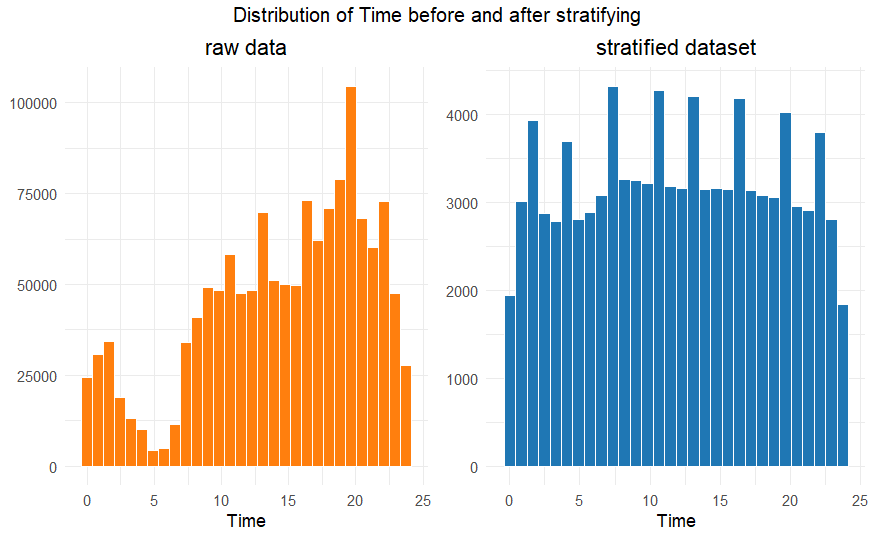
\includegraphics[keepaspectratio]{finalreport_files/stratified.png}}

\subsubsection{dataset sizes}\label{dataset-sizes}

There were different sizes of datasets created to allow for quicker
training of the model and extensive testing. In total four datasets were
created with 10.000, 50.000, 100.000 and 500.000 rows.

\newpage

\subsection{Model training and
evaluation}\label{model-training-and-evaluation}

With the stratified datasets in place the model training was able to
commence.

All models were trained and tested on the same datasets with the same
train/test splits to ensure a fair comparison.

The model were evaluated based on common metrics for regression models
such as root mean squared error, R² and the mean absolute error, as well
as the metrics root mean square error per 10 minutes and mean absolute
error in percent which the team has set as their own goals.

In the following table the results of the training, testing and
validating can be found for the best result for each model.

\begin{longtable}[]{@{}llllll@{}}
\toprule\noalign{}
Model & RMSE & MAE & R² & RMSE per 10 minutes & MAE in \% \\
\midrule\noalign{}
\endhead
\bottomrule\noalign{}
\endlastfoot
LM & 1.43 & 0.63 & 0.81 & 0.71 & 5.83 \\
GLM & 1.43 & 0.63 & 0.81 & 0.71 & 5.83 \\
XGBOOST & 0.82 & 0.35 & 0.94 & 0.41 & 3.03 \\
RF & 0.8 & 0.42 & 0.93 & 0.8 & 4.04 \\
NN & 1.27 & 0.64 & 0.83 & 1.27 & 6.63 \\
\end{longtable}

Plotting the results of one of the models reveals higher error margin
with shorter trips. As well as less accurate model predictions with
larger datasets.

\pandocbounded{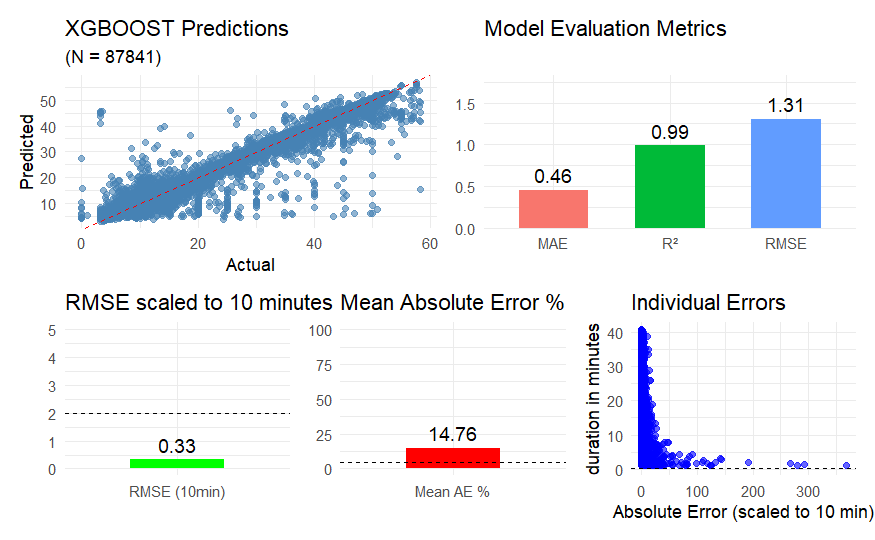
\includegraphics[keepaspectratio]{finalreport_files/xgboost_L.png}}

In this case the XGBOOST over prices the fares for smaller amounts and
under prices the fares for higher amounts. Therefore going for an
average between the two extremes. It still achieves the set goal for the
RMSE scaled to 10 minutes but fails to achieve and MAE in \% below 5
Percent.

Scaling the test and train data revealed no better metrics. The RMSE (10
min) as well as the Mean AE \% increased slightly.

\pandocbounded{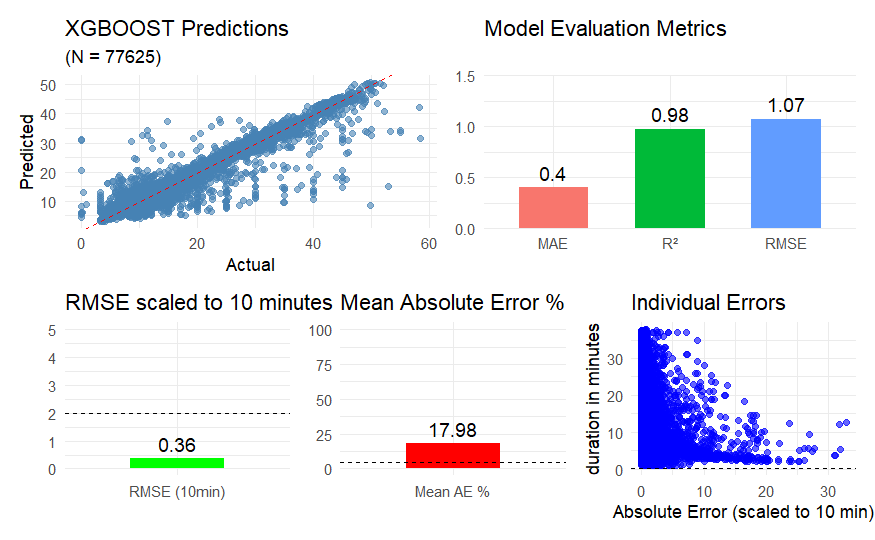
\includegraphics[keepaspectratio]{finalreport_files/xgboost_L_Scaled.png}}

\subsection{Model selection}\label{model-selection}

Although none of the model have reached the expected goals consistantly
over all dataset sizes, XGBoost has come closest. In the smallest
datasets it has reached both goals of an RMSE per 10 minutes smaller
than 2 and the MAE in \% smaller than 5. Therefor XGBoost was choosen as
the model to be used in the prototype.

\subsection{Shiny App}\label{shiny-app}

To create a prototype for users to select pickup and dropoff positions,
the shiny framework was used. A user has the possibility to add
coordinates and calculate their fare. The prototype also visualizes the
path which was calculated using open street maps.

\subsubsection{The shiny app when
opened}\label{the-shiny-app-when-opened}

\pandocbounded{\includegraphics[keepaspectratio]{.pdf}}

\pandocbounded{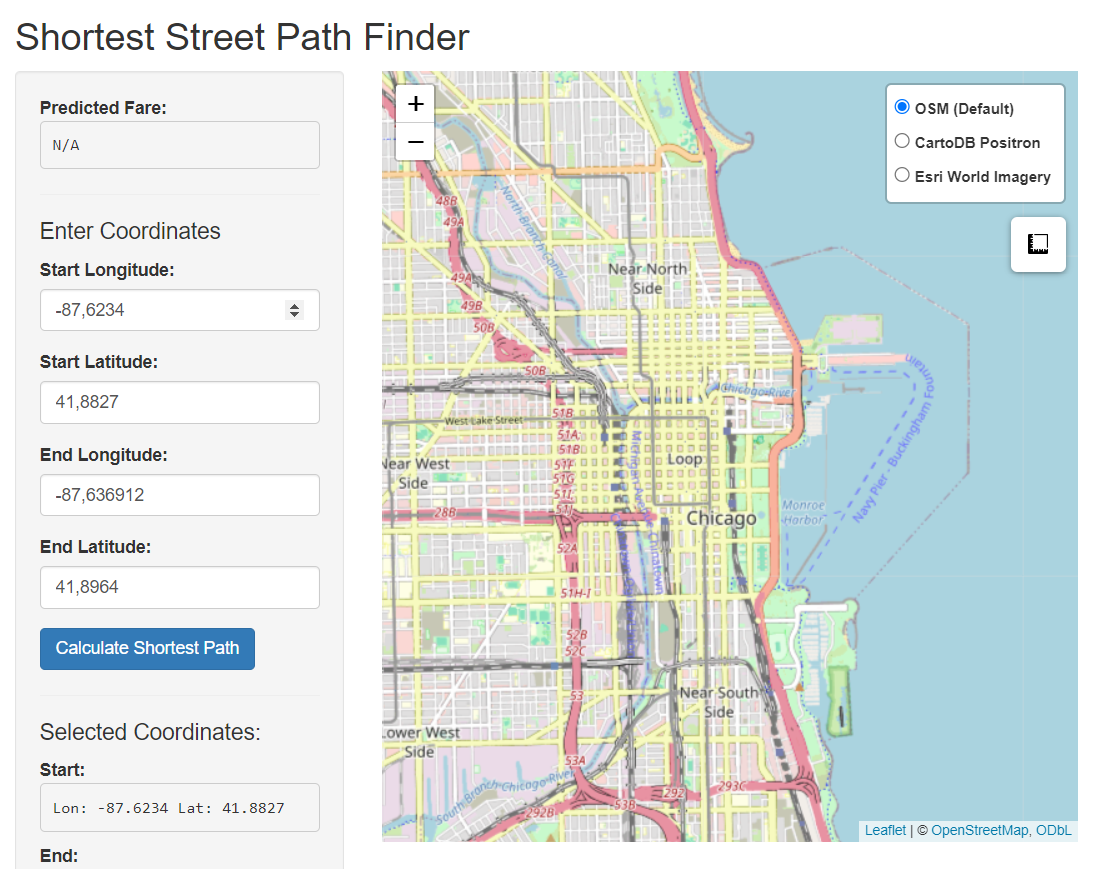
\includegraphics[keepaspectratio]{finalreport_files/emptyShiny.png}}

\newpage

\subsubsection{The shiny app when a path is
calculated}\label{the-shiny-app-when-a-path-is-calculated}

\pandocbounded{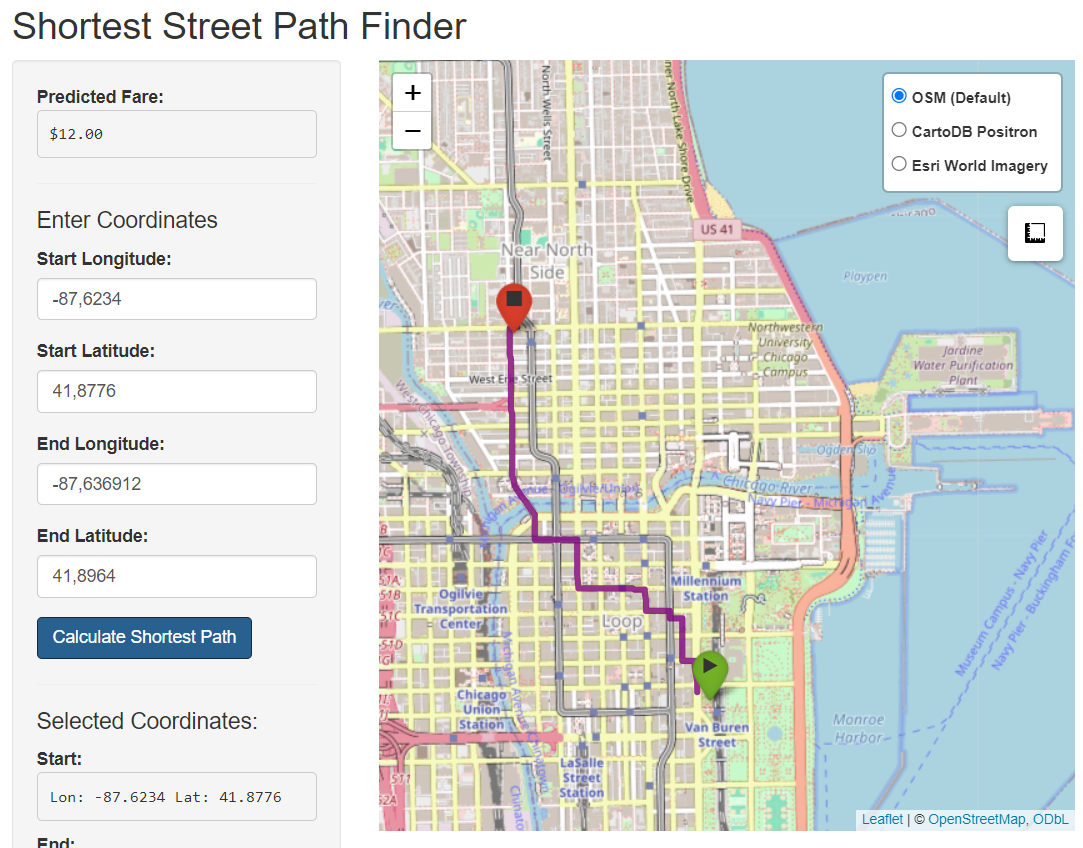
\includegraphics[keepaspectratio]{finalreport_files/path.png}}

\subsection{Conclusion}\label{conclusion}

This project has shown that multiple different model can be used for the
task of fare prediction. XGBoost has been shown to be the most accurate
on this particular dataset however the other models such as Random
Forrest or Neural networks could be fine tuned to achieve the same
metrics. However the training for those two models takes significantly
longer than for XGBoost.




\end{document}
